%
% 6.S077 problem set solutions template
%
\documentclass[12pt,twoside]{article}
\usepackage{bbm}

\newcommand{\name}{}

\usepackage{amssymb}
\usepackage{amsmath}
\usepackage{graphicx}
\usepackage{latexsym}
\usepackage{times,url}
\usepackage{cprotect}
\usepackage{listings}
\usepackage{graphicx}
\usepackage[table]{xcolor}
\usepackage[letterpaper]{geometry}
\usepackage{tikz-qtree}
\usepackage{enumerate}

\newcommand{\profs}{Mauricio Karchmer, Aleksander Madry, Bruce Tidor}
\newcommand{\subj}{6.046}
\newcommand{\ttt}[1]{{\tt\small #1}}

\definecolor{dkgreen}{rgb}{0,0.6,0}
\definecolor{gray}{rgb}{0.5,0.5,0.5}
\definecolor{mauve}{rgb}{0.58,0,0.82}

\lstset{
  language=Python,
  aboveskip=1pc,
  belowskip=1pc,
  basicstyle={\footnotesize\ttfamily},
  numbers=left,
  showstringspaces=false,
  numberstyle=\tiny\color{gray},
  keywordstyle=\color{blue},
  commentstyle=\color{dkgreen},
  stringstyle=\color{mauve},
}

\tikzset{
  % every node/.style={minimum width=2em,draw,circle},
  % level 1/.style={sibling distance=2cm},
  level distance=1cm,
  edge from parent/.style=
  {draw,edge from parent path={(\tikzparentnode) -- (\tikzchildnode)}},
}

\newif\ifHideSolutions
\newcommand{\solution}[1]{\color{dkgreen}\textbf{Solution: }#1\color{black}}
\newcommand{\rubric}[1]{\color{dkgreen}{\bf Rubric:} #1\color{black}}

% \HideSolutionsfalse
% \ifHideSolutions
%   \renewcommand{\solution}[1]{}
%   \renewcommand{\rubric}[1]{}
% \fi

\newlength{\toppush}
\setlength{\toppush}{2\headheight}
\addtolength{\toppush}{\headsep}

\newcommand{\htitle}[2]{\noindent\vspace*{-\toppush}\newline\parbox{6.5in}
{\textit{Design and Analysis of Algorithms}\hfill\name\newline
Massachusetts Institute of Technology \hfill #2\newline
\profs\hfill #1 \vspace*{-.5ex}\newline
\mbox{}\hrulefill\mbox{}}\vspace*{1ex}\mbox{}\newline
\begin{center}{\Large\bf #1}\end{center}}

\newcommand{\handout}[2]{\thispagestyle{empty}
 \markboth{#1}{#1}
 \pagestyle{myheadings}\htitle{#1}{#2}}

\newcommand{\lecture}[3]{\thispagestyle{empty}
 \markboth{Lecture #1: #2}{Lecture #1: #2}
 \pagestyle{myheadings}\htitle{Lecture #1: #2}{#3}}

\newcommand{\htitlewithouttitle}[2]{\noindent\vspace*{-\toppush}\newline\parbox{6.5in}
{\textit{Design and Analysis of Algorithms}\hfill#2\newline
Massachusetts Institute of Technology \hfill 6.046\newline
\profs\hfill Handout #1\vspace*{-.5ex}\newline
\mbox{}\hrulefill\mbox{}}\vspace*{1ex}\mbox{}\newline}

\newcommand{\handoutwithouttitle}[2]{\thispagestyle{empty}
 \markboth{Handout \protect\ref{#1}}{Handout \protect\ref{#1}}
 \pagestyle{myheadings}\htitlewithouttitle{\protect\ref{#1}}{#2}}

\newcommand{\exam}[2]{% parameters: exam name, date
 \thispagestyle{empty}
 \markboth{\hspace{1cm}\subj\ #1\hspace{1in}Name\hrulefill\ \ }%
          {\subj\ #1\hspace{1in}Name\hrulefill\ \ }
 \pagestyle{myheadings}\examtitle{#1}{#2}
 \renewcommand{\theproblem}{Problem \arabic{problemnum}}
}
\newcommand{\examsolutions}[3]{% parameters: handout, exam name, date
 \thispagestyle{empty}
 \markboth{Handout \protect\ref{#1}: #2}{Handout \protect\ref{#1}: #2}
% \pagestyle{myheadings}\htitle{\protect\ref{#1}}{#2}{#3}
 \pagestyle{myheadings}\examsolutionstitle{\protect\ref{#1}} {#2}{#3}
 \renewcommand{\theproblem}{Problem \arabic{problemnum}}
}
\newcommand{\examsolutionstitle}[3]{\noindent\vspace*{-\toppush}\newline\parbox{6.5in}
{\textit{Design and Analysis of Algorithms}\hfill#3\newline
Massachusetts Institute of Technology \hfill 6.046\newline
%Singapore-MIT Alliance \hfill SMA5503\newline
\profs\hfill Handout #1\vspace*{-.5ex}\newline
\mbox{}\hrulefill\mbox{}}\vspace*{1ex}\mbox{}\newline
\begin{center}{\Large\bf #2}\end{center}}

\newcommand{\takehomeexam}[2]{% parameters: exam name, date
 \thispagestyle{empty}
 \markboth{\subj\ #1\hfill}{\subj\ #1\hfill}
 \pagestyle{myheadings}\examtitle{#1}{#2}
 \renewcommand{\theproblem}{Problem \arabic{problemnum}}
}

\makeatletter
\newcommand{\exambooklet}[2]{% parameters: exam name, date
 \thispagestyle{empty}
 \markboth{\subj\ #1}{\subj\ #1}
 \pagestyle{myheadings}\examtitle{#1}{#2}
 \renewcommand{\theproblem}{Problem \arabic{problemnum}}
 \renewcommand{\problem}{\newpage
 \item \let\@currentlabel=\theproblem
 \markboth{\subj\ #1, \theproblem}{\subj\ #1, \theproblem}}
}
\makeatother


\newcommand{\examtitle}[2]{\noindent\vspace*{-\toppush}\newline\parbox{6.5in}
{\textit{Design and Analysis of Algorithms}\hfill#2\newline
Massachusetts Institute of Technology \hfill 6.046 Spring 2019\newline
%Singapore-MIT Alliance \hfill SMA5503\newline
\profs\hfill #1\vspace*{-.5ex}\newline
\mbox{}\hrulefill\mbox{}}\vspace*{1ex}\mbox{}\newline
\begin{center}{\Large\bf #1}\end{center}}

\newcommand{\grader}[1]{\hspace{1cm}\textsf{\textbf{#1}}\hspace{1cm}}

\newcommand{\points}[1]{[#1 points]\ }
\newcommand{\parts}[1]
{
  \ifnum#1=1
  (1 part)
  \else
  (#1 parts)
  \fi
  \ 
}

\newcommand{\bparts}{\begin{problemparts}}
\newcommand{\eparts}{\end{problemparts}}
\newcommand{\ppart}{\problempart}

%\newcommand{\lg} {lg\ }

\setlength{\oddsidemargin}{0pt}
\setlength{\evensidemargin}{0pt}
\setlength{\textwidth}{6.5in}
\setlength{\topmargin}{0in}
\setlength{\textheight}{8.5in}


\newcommand{\Spawn}{{\bf spawn} }
\newcommand{\Sync}{{\bf sync}}

\newcommand{\cif}[1]{\mbox{if $#1$}}
\newcommand{\cwhen}[1]{\mbox{when $#1$}}

\newcounter{problemnum}
\newcommand{\theproblem}{Problem \theproblemsetnum-\arabic{problemnum}}
\newenvironment{problems}{
        \begin{list}{{\bf \theproblem. \hspace*{0.5em}}}
        {\setlength{\leftmargin}{0em}
         \setlength{\rightmargin}{0em}
         \setlength{\labelwidth}{0em}
         \setlength{\labelsep}{0em}
         \usecounter{problemnum}}}{\end{list}}
\makeatletter
\newcommand{\problem}[1][{}]{\item \let\@currentlabel=\theproblem \textbf{#1}}
\makeatother

\newcounter{problempartnum}[problemnum]
\newenvironment{problemparts}{
        \begin{list}{{\bf (\alph{problempartnum})}}
        {\setlength{\leftmargin}{2.5em}
         \setlength{\rightmargin}{2.5em}
         \setlength{\labelsep}{0.5em}}}{\end{list}}
\newcommand{\problempart}{\addtocounter{problempartnum}{1}\item}

\newenvironment{truefalseproblemparts}{
        \begin{list}{{\bf (\alph{problempartnum})\ \ \ T\ \ F\hfil}}
        {\setlength{\leftmargin}{4.5em}
         \setlength{\rightmargin}{2.5em}
         \setlength{\labelsep}{0.5em}
         \setlength{\labelwidth}{4.5em}}}{\end{list}}

\newcounter{exercisenum}
\newcommand{\theexercise}{Exercise \theproblemsetnum-\arabic{exercisenum}}
\newenvironment{exercises}{
        \begin{list}{{\bf \theexercise. \hspace*{0.5em}}}
        {\setlength{\leftmargin}{0em}
         \setlength{\rightmargin}{0em}
         \setlength{\labelwidth}{0em}
         \setlength{\labelsep}{0em}
        \usecounter{exercisenum}}}{\end{list}}
\makeatletter
\newcommand{\exercise}{\item \let\@currentlabel=\theexercise}
\makeatother

\newcounter{exercisepartnum}[exercisenum]
%\newcommand{\problem}[1]{\medskip\mbox{}\newline\noindent{\bf Problem #1.}\hspace*{1em}}
%\newcommand{\exercise}[1]{\medskip\mbox{}\newline\noindent{\bf Exercise #1.}\hspace*{1em}}

\newenvironment{exerciseparts}{
        \begin{list}{{\bf (\alph{exercisepartnum})}}
        {\setlength{\leftmargin}{2.5em}
         \setlength{\rightmargin}{2.5em}
         \setlength{\labelsep}{0.5em}}}{\end{list}}
\newcommand{\exercisepart}{\addtocounter{exercisepartnum}{1}\item}


% Macros to make captions print with small type and 'Figure xx' in bold.
\makeatletter
\def\fnum@figure{{\bf Figure \thefigure}}
\def\fnum@table{{\bf Table \thetable}}
\let\@mycaption\caption
%\long\def\@mycaption#1[#2]#3{\addcontentsline{\csname
%  ext@#1\endcsname}{#1}{\protect\numberline{\csname 
%  the#1\endcsname}{\ignorespaces #2}}\par
%  \begingroup
%    \@parboxrestore
%    \small
%    \@makecaption{\csname fnum@#1\endcsname}{\ignorespaces #3}\par
%  \endgroup}
%\def\mycaption{\refstepcounter\@captype \@dblarg{\@mycaption\@captype}}
%\makeatother
\let\mycaption\caption
%\newcommand{\figcaption}[1]{\mycaption[]{#1}}

\newcounter{totalcaptions}
\newcounter{totalart}

\newcommand{\figcaption}[1]{\addtocounter{totalcaptions}{1}\caption[]{#1}}

% \psfigures determines what to do for figures:
%       0 means just leave vertical space
%       1 means put a vertical rule and the figure name
%       2 means insert the PostScript version of the figure
%       3 means put the figure name flush left or right
\newcommand{\psfigures}{0}
\newcommand{\spacefigures}{\renewcommand{\psfigures}{0}}
\newcommand{\rulefigures}{\renewcommand{\psfigures}{1}}
\newcommand{\macfigures}{\renewcommand{\psfigures}{2}}
\newcommand{\namefigures}{\renewcommand{\psfigures}{3}}

\newcommand{\figpart}[1]{{\bf (#1)}\nolinebreak[2]\relax}
\newcommand{\figparts}[2]{{\bf (#1)--(#2)}\nolinebreak[2]\relax}


\macfigures     % STATE

% When calling \figspace, make sure to leave a blank line afterward!!
% \widefigspace is for figures that are more than 28pc wide.
\newlength{\halffigspace} \newlength{\wholefigspace}
\newlength{\figruleheight} \newlength{\figgap}
\newcommand{\setfiglengths}{\ifnum\psfigures=1\setlength{\figruleheight}{\hruleheight}\setlength{\figgap}{1em}\else\setlength{\figruleheight}{0pt}\setlength{\figgap}{0em}\fi}
\newcommand{\figspace}[2]{\ifnum\psfigures=0\leavefigspace{#1}\else%
\setfiglengths%
\setlength{\wholefigspace}{#1}\setlength{\halffigspace}{.5\wholefigspace}%
\rule[-\halffigspace]{\figruleheight}{\wholefigspace}\hspace{\figgap}#2\fi}
\newlength{\widefigspacewidth}
% Make \widefigspace put the figure flush right on the text page.
\newcommand{\widefigspace}[2]{
\ifnum\psfigures=0\leavefigspace{#1}\else%
\setfiglengths%
\setlength{\widefigspacewidth}{28pc}%
\addtolength{\widefigspacewidth}{-\figruleheight}%
\setlength{\wholefigspace}{#1}\setlength{\halffigspace}{.5\wholefigspace}%
\makebox[\widefigspacewidth][r]{#2\hspace{\figgap}}\rule[-\halffigspace]{\figruleheight}{\wholefigspace}\fi}
\newcommand{\leavefigspace}[1]{\setlength{\wholefigspace}{#1}\setlength{\halffigspace}{.5\wholefigspace}\rule[-\halffigspace]{0em}{\wholefigspace}}

% Commands for including figures with macpsfig.
% To use these commands, documentstyle ``macpsfig'' must be specified.
\newlength{\macfigfill}
\makeatother
\newlength{\bbx}
\newlength{\bby}
\newcommand{\macfigure}[5]{\addtocounter{totalart}{1}
\ifnum\psfigures=2%
\setlength{\bbx}{#2}\addtolength{\bbx}{#4}%
\setlength{\bby}{#3}\addtolength{\bby}{#5}%
\begin{flushleft}
\ifdim#4>28pc\setlength{\macfigfill}{#4}\addtolength{\macfigfill}{-28pc}\hspace*{-\macfigfill}\fi%
\mbox{\psfig{figure=./#1.ps,%
bbllx=#2,bblly=#3,bburx=\bbx,bbury=\bby}}
\end{flushleft}%
\else\ifdim#4>28pc\widefigspace{#5}{#1}\else\figspace{#5}{#1}\fi\fi}
\makeatletter

\newlength{\savearraycolsep}
\newcommand{\narrowarray}[1]{\setlength{\savearraycolsep}{\arraycolsep}\setlength{\arraycolsep}{#1\arraycolsep}}
\newcommand{\normalarray}{\setlength{\arraycolsep}{\savearraycolsep}}

\newcommand{\hint}{{\em Hint:\ }}

% Macros from /th/u/clr/mac.tex

\newcommand{\set}[1]{\left\{ #1 \right\}}
\newcommand{\abs}[1]{\left| #1\right|}
\newcommand{\card}[1]{\left| #1\right|}
\newcommand{\floor}[1]{\left\lfloor #1 \right\rfloor}
\newcommand{\ceil}[1]{\left\lceil #1 \right\rceil}
\newcommand{\ang}[1]{\ifmmode{\left\langle #1 \right\rangle}
   \else{$\left\langle${#1}$\right\rangle$}\fi}
        % the \if allows use outside mathmode,
        % but will swallow following space there!
\newcommand{\paren}[1]{\left( #1 \right)}
\newcommand{\bracket}[1]{\left[ #1 \right]}
\newcommand{\prob}[1]{\Pr\left\{ #1 \right\}}
\newcommand{\Var}{\mathop{\rm Var}\nolimits}
\newcommand{\expect}[1]{{\rm E}\left[ #1 \right]}
\newcommand{\expectsq}[1]{{\rm E}^2\left[ #1 \right]}
\newcommand{\variance}[1]{{\rm Var}\left[ #1 \right]}
\renewcommand{\choose}[2]{{{#1}\atopwithdelims(){#2}}}
\def\pmod#1{\allowbreak\mkern12mu({\rm mod}\,\,#1)}
\newcommand{\matx}[2]{\left(\begin{array}{*{#1}{c}}#2\end{array}\right)}
\newcommand{\Adj}{\mathop{\rm Adj}\nolimits}

\newtheorem{theorem}{Theorem}
\newtheorem{lemma}[theorem]{Lemma}
\newtheorem{corollary}[theorem]{Corollary}
\newtheorem{xample}{Example}
\newtheorem{definition}{Definition}
\newenvironment{example}{\begin{xample}\rm}{\end{xample}}
\newcommand{\proof}{\noindent{\em Proof.}\hspace{1em}}
\def\squarebox#1{\hbox to #1{\hfill\vbox to #1{\vfill}}}
\newcommand{\qedbox}{\vbox{\hrule\hbox{\vrule\squarebox{.667em}\vrule}\hrule}}
\newcommand{\qed}{\nopagebreak\mbox{}\hfill\qedbox\smallskip}
\newcommand{\eqnref}[1]{(\protect\ref{#1})}

%%\newcommand{\twodots}{\mathinner{\ldotp\ldotp}}
\newcommand{\transpose}{^{\mbox{\scriptsize \sf T}}}
\newcommand{\amortized}[1]{\widehat{#1}}

\newcommand{\punt}[1]{}

%%% command for putting definitions into boldface
% New style for defined terms, as of 2/23/88, redefined by THC.
\newcommand{\defn}[1]{{\boldmath\textit{\textbf{#1}}}}
\newcommand{\defi}[1]{{\textit{\textbf{#1\/}}}}

\newcommand{\red}{\leq_{\rm P}}
\newcommand{\lang}[1]{%
\ifmmode\mathord{\mathcode`-="702D\rm#1\mathcode`\-="2200}\else{\rm#1}\fi}

%\newcommand{\ckt}[1]{\ifmmode\mathord{\mathcode`-="702D\sc #1\mathcode`\-="2200}\else$\mathord{\mathcode`-="702D\sc #1\mathcode`\-="2200}$\fi}
\newcommand{\ckt}[1]{\ifmmode \sc #1\else$\sc #1$\fi}

%% Margin notes - use \notesfalse to turn off notes.
\setlength{\marginparwidth}{0.6in}
\reversemarginpar
\newif\ifnotes
\notestrue
\newcommand{\longnote}[1]{
  \ifnotes
    {\medskip\noindent Note: \marginpar[\hfill$\Longrightarrow$]
      {$\Longleftarrow$}{#1}\medskip}
  \fi}
\newcommand{\note}[1]{
  \ifnotes
    {\marginpar{\tiny \raggedright{#1}}}
  \fi}


\newcommand{\reals}{\mathbbm{R}}
\newcommand{\integers}{\mathbbm{Z}}
\newcommand{\naturals}{\mathbbm{N}}
\newcommand{\rationals}{\mathbbm{Q}}
\newcommand{\complex}{\mathbbm{C}}

\newcommand{\oldreals}{{\bf R}}
\newcommand{\oldintegers}{{\bf Z}}
\newcommand{\oldnaturals}{{\bf N}}
\newcommand{\oldrationals}{{\bf Q}}
\newcommand{\oldcomplex}{{\bf C}}

\newcommand{\w}{\omega}                 %% for fft chapter

\newenvironment{closeitemize}{\begin{list}
{$\bullet$}
{\setlength{\itemsep}{-0.2\baselineskip}
\setlength{\topsep}{0.2\baselineskip}
\setlength{\parskip}{0pt}}}
{\end{list}}

% These are necessary within a {problems} environment in order to restore
% the default separation between bullets and items.
\newenvironment{normalitemize}{\setlength{\labelsep}{0.5em}\begin{itemize}}
                              {\end{itemize}}
\newenvironment{normalenumerate}{\setlength{\labelsep}{0.5em}\begin{enumerate}}
                                {\end{enumerate}}

%\def\eqref#1{Equation~(\ref{eq:#1})}
%\newcommand{\eqref}[1]{Equation (\ref{eq:#1})}
\newcommand{\eqreftwo}[2]{Equations (\ref{eq:#1}) and~(\ref{eq:#2})}
\newcommand{\ineqref}[1]{Inequality~(\ref{ineq:#1})}
\newcommand{\ineqreftwo}[2]{Inequalities (\ref{ineq:#1}) and~(\ref{ineq:#2})}

\newcommand{\figref}[1]{Figure~\ref{fig:#1}}
\newcommand{\figreftwo}[2]{Figures \ref{fig:#1} and~\ref{fig:#2}}

\newcommand{\liref}[1]{line~\ref{li:#1}}
\newcommand{\Liref}[1]{Line~\ref{li:#1}}
\newcommand{\lirefs}[2]{lines \ref{li:#1}--\ref{li:#2}}
\newcommand{\Lirefs}[2]{Lines \ref{li:#1}--\ref{li:#2}}
\newcommand{\lireftwo}[2]{lines \ref{li:#1} and~\ref{li:#2}}
\newcommand{\lirefthree}[3]{lines \ref{li:#1}, \ref{li:#2}, and~\ref{li:#3}}

\newcommand{\lemlabel}[1]{\label{lem:#1}}
\newcommand{\lemref}[1]{Lemma~\ref{lem:#1}} 

\newcommand{\exref}[1]{Exercise~\ref{ex:#1}}

\newcommand{\handref}[1]{Handout~\ref{#1}}

\newcommand{\defref}[1]{Definition~\ref{def:#1}}

% (1997.8.16: Victor Luchangco)
% Modified \hlabel to only get date and to use handouts counter for number.
%   New \handout and \handoutwithouttitle commands in newmac.tex use this.
%   The date is referenced by <label>-date.
%   (Retained old definition as \hlabelold.)
%   Defined \hforcelabel to use an argument instead of the handouts counter.

\newcounter{handouts}
\setcounter{handouts}{0}

\newcommand{\hlabel}[2]{%
\stepcounter{handouts}
{\edef\next{\write\@auxout{\string\newlabel{#1}{{\arabic{handouts}}{0}}}}\next}
\write\@auxout{\string\newlabel{#1-date}{{#2}{0}}}
}

\newcommand{\hforcelabel}[3]{%          Does not step handouts counter.
\write\@auxout{\string\newlabel{#1}{{#2}{0}}}
\write\@auxout{\string\newlabel{#1-date}{{#3}{0}}}}


% less ugly underscore
% --juang, 2008 oct 05
\renewcommand{\_}{\vrule height 0 pt depth 0.4 pt width 0.5 em \,}

\newcommand{\theproblemsetnum}{1}
\newcommand{\releasedate}{Thursday, February 7}
\newcommand{\partaduedate}{Thursday, February 14}

\title{6.S077 Problem Set \theproblemsetnum}

\begin{document}

\handout{Problem Set \theproblemsetnum}{\releasedate}
\textbf{All parts are due {\bf \partaduedate} at {\bf 2:30PM}}.

\setlength{\parindent}{0pt}
\medskip\hrulefill\medskip

{\bf Name:} Robert Durfee

\medskip

{\bf Collaborators:} None

\medskip\hrulefill

\begin{problems}

\problem  % Problem 1

\begin{problemparts}

\problempart % Problem 1a

%%%%%%%%%%%%%%%%%%%%%%%%%%%%%%%%%%%%%%%%%%%%%%%%%%%%%%%%%%%%%%%%%%%%%%%%%%%%%%%%
An equivalent way to express the Weak Law of Large Numbers is,
$$\lim_{n \to \infty} \mathbb{P}\left(\vert \hat{P}_i - p_i \vert > \varepsilon
\right) = 0\quad \forall i $$
Boole's inequality states,
$$ \mathbb{P}\left(\bigcup_i A_i\right) \leq \sum_i \mathbb{P}(A_i) $$
Thus, we can show that all $\hat{P}_i$ approach $p_i$ simultaneously,
$$ \mathbb{P}\left(\bigcup_i \vert \hat{P}_i - p_i \vert > \varepsilon \right) 
\leq \sum_i \mathbb{P} \left(\vert \hat{P}_i - p_i \vert > \varepsilon \right) $$
But we know that the right hand side must be zero because of the Weak Law of
Large Numbers. Therefore,
$$ \mathbb{P}\left(\bigcup_i \vert \hat{P}_i - p_i \vert > \varepsilon \right) 
= 0 $$
Which is equivalent to
$$ \mathbb{P} \left( \vert \hat{P}_i - p_i \vert \leq \varepsilon, \ \forall 
i \right) = 1 $$

\problempart % Problem 1b

Let $\mathbbm{1}_i(x)$ be the indicator random variable with the following
distribution,
$$ \mathbbm{1}_i(x) = \begin{cases}
    1 & \mathrm{if}\ X_i \leq x \\
    0 & \mathrm{if}\ X_i > x
\end{cases} $$
Then, the definition of the empirical CDF can be written as
$$ \hat{F}(x) = \frac{\sum_i \mathbbm{1}_i(x)}{n} $$
From Chebyshev's inequality, we know,
$$ \mathbb{P}\left(\left\vert \frac{\sum_i \mathbbm{1}_i(x)}{n} - \mathbb{F}(x)
\right\vert > \varepsilon\right) \leq \frac{\mathrm{var}\left(\sum_i 
\mathbbm{1}_i(x) / n\right)}{\varepsilon^2} $$
Since $X$ is i.i.d., the variance of the empirical distribution can be written,
$$ \mathrm{var}\left(\frac{\sum_i \mathbbm{1}_i(x)}{n}\right) = \frac{1}{n^2} 
\sum_i \mathrm{var} \left(\mathbbm{1}_i(x)\right) $$
And, the variance of the indicator random variable is given by
$$ \mathbbm{1}_i(x) = \mathbb{P}(X_i \leq x)\left(1 - \mathbb{P}(X_i \leq x)
\right) $$
Since $X$ are i.i.d., the subscripts can be removed,
$$ \mathbbm{1}(x) = \mathbb{P}(X \leq x)\left(1 - \mathbb{P}(X \leq x)
\right) $$
Now, the variance can be written,
$$\mathrm{var}(\hat{F}(x)) = \frac{\mathbb{P}(X \leq x)\left(1 - \mathbb{P}
(X \leq x) \right)}{n} $$
Substituting back into the inequality,
$$ \mathbb{P}\left(\left\vert \frac{\sum_i \mathbbm{1}_i(x)}{n} - \mathbb{F}(x)
\right\vert > \varepsilon\right) \leq \frac{\mathbb{P}(X \leq x)\left(1 - 
\mathbb{P}(X \leq x) \right)}{n \varepsilon^2} $$
And, as $n$ approaches infinity, the right hand side goes to zero,
$$ \mathbb{P}\left(\left\vert \hat{F}(x) - \mathbb{F}(x) \right\vert > 
\varepsilon\right) = 0$$




\end{problemparts}

\newpage
\problem  % Problem 2

\begin{problemparts}

\problempart % Problem 2a
%%%%%%%%%%%%%%%%%%%%%%%%%%%%%%%%%%%%%%%%%%%%%%%%%%%%%%%%%%%%%%%%%%%%%%%%%%%%%%%%
Since $X_1, X_2, \ldots, X_n$ are independent, the joint distribution is given
by multiplying the individual terms together,
$$ f_{X_1\ldots X_n}^\theta(x_1, \ldots, x_n) = \prod_{i = 1}^n \theta e^{-
\theta x_i} $$
Taking the natural logarithm of both sides,
$$ \ln f_{X_1\ldots X_n}^\theta(x_1, \ldots, x_n) = \sum_{i = 1}^n \left(\ln 
\theta - \theta x_i\right) $$
Breaking the sum apart,
$$ \ln f_{X_1\ldots X_n}^\theta(x_1, \ldots, x_n) = n \ln \theta - \theta 
\sum_{i = 1}^n x_i $$
Taking the derivative with respect to $\theta$ and setting equal to zero,
$$ 0 = \frac{n}{\hat{\theta}} - \sum_{i = 1}^n x_i $$
Solving for $\hat{\theta}$ yields,
$$ \hat{\theta} = \frac{n}{\sum_{i = 1}^n x_i} $$

\problempart % Problem 2b
%%%%%%%%%%%%%%%%%%%%%%%%%%%%%%%%%%%%%%%%%%%%%%%%%%%%%%%%%%%%%%%%%%%%%%%%%%%%%%%%
We determine the empirical first moment from the observations,
$$ \hat{\mathbb{E}}[X] = \frac{1}{n} \sum_{i = 1}^n x_i $$
The first moment of the model dependent upon $\theta_1$ is given by the
definition of the mean of an exponential distribution,
$$ \mathbb{E}[X] = \frac{1}{\theta_1} $$
Equating these two equations and solving for $\hat{\theta}_1$,
$$ \hat{\theta}_1 = \frac{n}{\sum_{i = 1}^n x_i} $$

Now we determine the empirical second moment from the observations,
$$ \hat{\mathbb{E}}[X^2] = \frac{1}{n} \sum_{i = 1}^n x_i^2 $$
The second moment of the model dependent upon $\theta_2$ is given through the
definition of the variance of an exponential distribution,
$$ \mathbb{E}[X^2] = \mathrm{var}(X) + \mathbb{E}[X]^2 = \frac{2}{\theta_2} $$
Equating these two equations and solving for $\hat{\theta}_2$,
$$ \hat{\theta}_2 = \sqrt{\frac{2n}{\sum_{i = 1}^n x_i^2}} $$

\problempart % Problem 2c
%%%%%%%%%%%%%%%%%%%%%%%%%%%%%%%%%%%%%%%%%%%%%%%%%%%%%%%%%%%%%%%%%%%%%%%%%%%%%%%%
The definition of the median provided,
$$ \mathbb{P}(X \leq a_\theta) = \frac{1}{2} $$
This can be written in terms of the CDF,
$$ F_X(a_\theta) = \frac{1}{2} $$ 
The CDF for an exponential distribution is known, thus this becomes,
$$ 1 - e^{-\theta a_\theta} = \frac{1}{2} $$
Solving for $a_\theta$ yields,
$$ a_\theta = -\frac{\ln(1/2)}{\theta} = \frac{\ln 2}{\theta} $$

Given the empirical median $\hat{a}$, we can form an estimate of $\theta$ with
feature matching,
$$ \hat{a} = \frac{\ln 2}{\hat{\theta}_m} $$
Solving for $\hat{\theta}_m$,
$$ \hat{\theta}_m = \frac{\ln 2}{\hat{a}} $$

\problempart % Problem 2d

See Jupyter Notebook for details. The results are provided below.

$$ \hat{\theta}_{ML} = 2.6235,\quad \hat{\theta}_{1} = 2.6235 $$
$$ \hat{\theta}_{2} = 2.8651,\quad \hat{\theta}_{m} = 2.4866 $$

\end{problemparts}

\newpage
\problem  % Problem 3

\begin{problemparts}

\problempart % Problem 3a
%%%%%%%%%%%%%%%%%%%%%%%%%%%%%%%%%%%%%%%%%%%%%%%%%%%%%%%%%%%%%%%%%%%%%%%%%%%%%%%%
The maximum likelihood function is of the form,
$$ f_{X_1\ldots X_n}(x_1, \ldots, x_n) = \prod_{i = 1}^n \frac{1}{\sqrt{2 \pi 
v}} e^{-(x_i - \mu)^2 / 2v} $$
Taking the natural logarithm of both sides and simplifying,
$$ \ln f_{X_1\ldots X_n}(x_1, \ldots, x_n) = n \ln \left(\frac{1}{\sqrt{2 \pi 
v}}\right) - \sum_{i = 1}^n \frac{(x_i - \mu)^2}{2v} $$

To determine the estimate for $\hat{\mu}$, take the partial derivative with
respect to $\mu$ and set to zero,
$$ 0 = \sum_{i = 1}^n \frac{x_i - \hat{\mu}}{v} = \sum_{i = 1}^n x_i - 
\hat{\mu} = \sum_{i = 1}^n x_i - n \hat{\mu} $$
Solving for $\hat{\mu}$
$$ \hat{\mu} = \frac{1}{n} \sum_{i = 1}^n x_i $$

To determine the estimate for $\hat{v}$, take the partial derivative with
respect to $v$ and set to zero,
$$ 0 = -\frac{n}{2\hat{v}} + \frac{1}{2 \hat{v}^2} \sum_{i = 1}^n (x_i - 
\hat{\mu})^2 = -n + \frac{1}{\hat{v}} \sum_{i = 1}^n (x_i - \hat{\mu})^2 $$
Solving for $\hat{v}$,
$$ \hat{v} = \frac{1}{n} \sum_{i = 1}^n (x_i - \hat{\mu})^2 $$

\problempart % Problem 3b

See Jupyter Notebook for details.

\begin{center}
    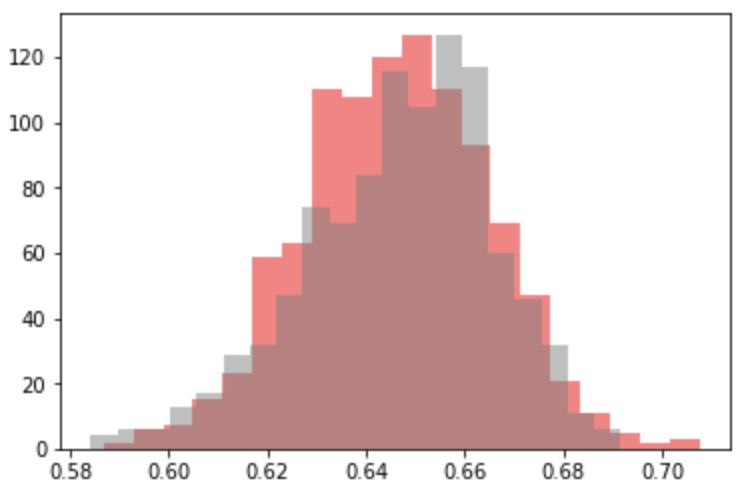
\includegraphics[scale=0.75]{PS1P3B.png}
\end{center}

\problempart % Problem 3c
%%%%%%%%%%%%%%%%%%%%%%%%%%%%%%%%%%%%%%%%%%%%%%%%%%%%%%%%%%%%%%%%%%%%%%%%%%%%%%%%
Considering a mixture of two Gaussian distributions, the distribution of a $X_i$
given a parameter vector $\theta$ would look like,
$$ f_{X_i}^\theta(x_i) = \frac{\lambda}{\sqrt{2 \pi v_1}} e^{-(x_i - \mu_1)^2 
/ 2 v_1} + \frac{1 - \lambda}{\sqrt{2 \pi v_2}} e^{-(x_i - \mu_2)^2 / 2 v_2} $$

\problempart % Problem 3d

When $v_1 \longrightarrow 0$, the likelihood approaches infinity. As a result,
there is no definite maximum value of $L^\theta$ when optimizing over $\theta$.

\problempart % Problem 3e

See Jupyter Notebook for details.

\begin{center}
    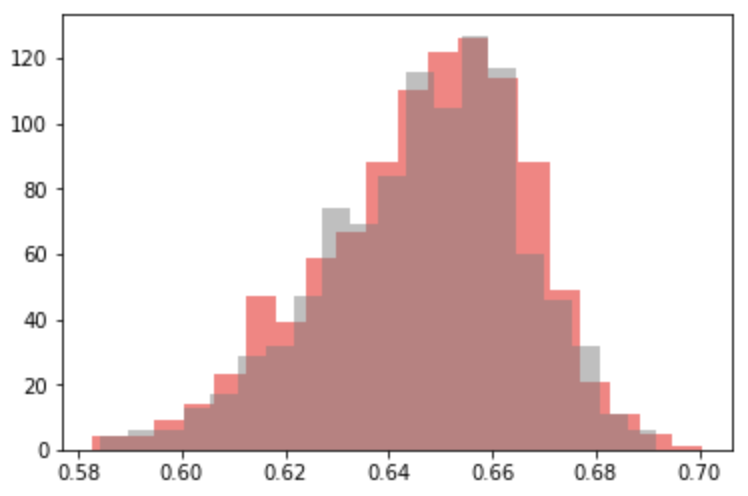
\includegraphics[scale=0.75]{PS1P3E.png}
\end{center}

\problempart % Problem 3f

See Jupyter Notebook for details. The results are provided below.

$$ \hat{\mathbb{E}}[X^1] = 0.6468,\quad \hat{\mathbb{E}}[X^2] = 0.4187,\quad
\hat{\mathbb{E}}[X^3] = 0.2712 $$
$$ \hat{\mathbb{E}}[X^4] = 0.1759,\quad \hat{\mathbb{E}}[X^5] = 0.1141 $$

\problempart % Problem 3g

The second moment of a normal random variable $Y$,
$$ \mathbb{E}[Y^2] = \mathbb{E}[(\mu + \sigma Z)^2] = \mathbb{E}[\mu^2 + 2 \mu 
\sigma Z  + \sigma^2 Z^2] = \mu^2 + \sigma^2 = \mu^2 + v $$
The third moment of a normal random variable $Y$,
$$ \mathbb{E}[Y^3] = \mathbb{E}[(\mu + \sigma Z)^2] = \mathbb{E}[\mu^3 + 3 
\mu^2 \sigma Z + 3 \mu \sigma^2 Z^2 + \sigma^3 Z^3] = \mu^3 + 3 \mu \sigma^2 =
\mu^3 + 3 \mu v $$

Using the moments for individual Gaussian random variables and the law of
total expectation, we can find the fifth moment of $X$, our mixture model. 
Let $\Lambda$ be the indicator random variable such that the first Gaussian 
is chosen when $\Lambda = 0$ with probability $\lambda$ and the second 
Gaussian is chosen when $\Lambda = 1$ with probability $1 - \lambda$. The
law of total expectation dictates,
$$ \mathbb{E}[X^5] = \lambda \mathbb{E}[X^5 \mid \Lambda = 0] + (1 - 
\lambda) \mathbb{E}[X^5 \mid \Lambda = 1] $$
Let $Y$ be the first Gaussian with $(\mu_1, v_1)$ and let $Z$ be the second
Gaussian with $(\mu_2, v_2)$. The equation simplifies,
$$ \mathbb{E}[X^5] = \lambda \mathbb{E}[Y^5] + (1 - \lambda) \mathbb{E}[Z^5] $$
From the definitions of the fifth moments of a Gaussian distribution,
$$ \mathbb{E}[X^5] = \lambda (\mu_1^5 + 10 \mu_1^3 v_1 + 15 \mu_1 v_1^2) + (1
- \lambda) (\mu_2^5 + 10 \mu_2^3 v_2 + 15 \mu_2 v_2^3) $$

\problempart % Problem 3h

If the evidence overwhelmingly suggests that two Gaussian distributions yielded
the results observed (and one realizes the fact that traits are exhibited within
populations normally), there are several explanations. One possibility might be
a difference between male and female traits. Another could be that two different
people did the measuring one was systematically worse at measuring than the other.
Or, perhaps, someone was maliciously attempting to ambush the study by altering
the data after-the-fact to make it look like to Gaussians were involved.

\end{problemparts}

\end{problems}

\end{document}


